\section{Routing Algorithms and IoT Based Evacuation Management}
\label{sec:pastwork:Routing Algorithms and IoT Based Evacuation Management}

Routing algorithms and maze solving algorithms have especially been applied to the structural domains for the real time analysis of shortest paths and obstacle avoidance by both machine and human agents since the time the earliest shortest paths algorithms were developed. The development of the shortest path algorithm by Dijkstra in 1956, especially has seen a plethora of applications in various fields. As one can guess most of its applications have been catered to graph based problems and obstacle avoidance. Shortest paths exit strategy formation approach is a good way to analyse a safe egress as it provides obstacle avoidance as well. How can it successfully be applied to a real disaster scenario? Before the advancements were made to IoT based infrastructure, maze solving algorithms were used to successfully analyze a safe egress. 

IoT and computation systems have brough about a tremendous potential to perceive the environment and then form the necessary strategies that are required to safely escort the human agents to a safe exit point during the time of disaster. Modern evacuation systems have sensors in place to allow for better perception of the world during a disaster scenario. For instance the work by Kobes et al. determined that during fire related disaster scenarios, 56.3\% of the participating agents were able to determine the exit points based on the exit signs when there was no smoke present whilst 81.8\% was able to identify exit points only based on the exit signs when their vision was imparied due to smoke [11]. Based on such data for instance, it greatly enhances our need to analyse the fastest and shortest egress path so that all human agents in the vicinity can get to the exit points. The shortest path algorithm - Dijkstra's algorithm is currently used as a great tool to provide the shortest exit points as it is demonstrated in the work by Jehyun Cho [12]. His research pertains to the dynamic analysis of a shortest path algorithm based on information obtained from the sensors and the smart infrastructure.  

In order to address the issue of agent(s) and infrastructure mapping during a disaster event, state of the art sensors are placed all through the infrastructure in order to perceive the environment and the surrounding structures in order to analyze a safe egress. Motion detectors for instance are used to understand how many people are still trapped inside the building during a catastrophe. One example of using IoT technologies is proposed by Prasad Annadata et al. using multiple WIFI channels and the aforementioned motion detectors [13]. Based on the statistics gathered heuristic solutions are proposed in order to detect the number of personnel inside the infrastructure as well as perceive the environment.          

% Everyone needs floating figures in their dissertation. 

% As shown in Figure~\ref{fig:pastwork:titlepage}, the Mudd Library dissertation requirements~\cite{muddthesis2009} specify additional options for formatting the title page. For example, if your thesis has multiple volumes, or to indicate the proper formatting for a master's thesis.

% \begin{figure}[htb]
%   \begin{center}
%     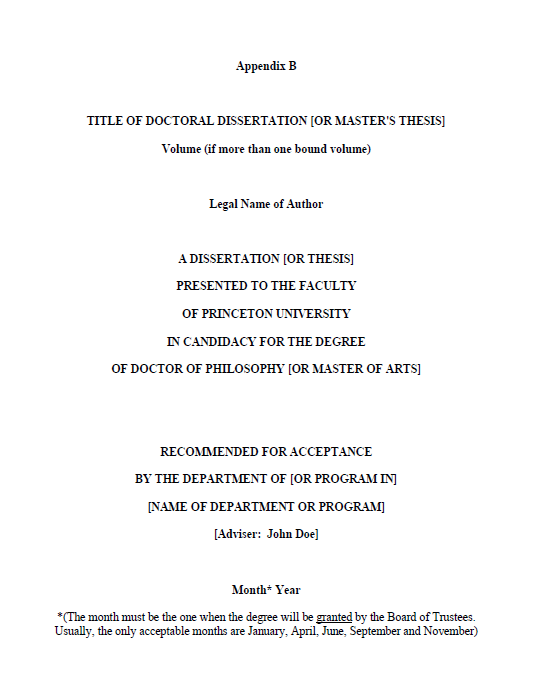
\includegraphics[width=0.9\linewidth]{ch-pastwork/figures/titlepage}
%     \caption[Sample Title Page Layout]{Sample title page layout~\cite{muddthesis2009}}
%     \label{fig:pastwork:titlepage}
%   \end{center}
% \end{figure}
